\section{Overview of Related Works}

\subsection{Unimodal Wearable Sensor-Based Approaches}
Single-channel wearable sensing remains a strong baseline and, importantly for the argument
developed here, frequently matches multimodal systems on public benchmarks. EDA is the most
direct peripheral index of sympathetic arousal and has been used alone for binary stress
classification across four public corpora \cite{r52} and in privacy-preserving federated
settings \cite{r72}. HRV derived from ECG supports stress classification in factory workers
\cite{r5}, physicians \cite{r1} and office employees \cite{r61}, and ECG-derived multifractal
descriptors have been proposed specifically to separate cognitive stress from physical
activity \cite{r56}.

PPG has attracted the most recent methodological attention because it is the channel
available on consumer hardware. Lightweight architectures operating on blood volume pulse
alone now report $98.23\%$ accuracy with an AUC of $0.9953$ on WESAD \cite{r50} and $96.94\%$
under leave-one-subject-out (LOSO) validation \cite{r55}, while a separable-attention dilated
network evaluated under LOSO across two cohorts reports $92.25\%$ \cite{r47}. In-ear PPG
transformed into time-frequency images and classified with a vision transformer reaches
$97.78\%$ \cite{r43}. EEG offers the greatest neurophysiological specificity, and miniaturised
behind-the-ear devices with on-chip inference have made it more practical \cite{r31},
although headset intrusiveness still limits naturalistic use.

The essential observation is that these unimodal systems are not obviously worse than the
multimodal systems they are implicitly compared against. That observation is the starting
point for the present analysis.

\subsection{Unimodal Computer Vision-Based Approaches}
Camera-based affect and attention sensing rests on facial expression analysis, gaze and blink
dynamics, head pose and camera-derived physiological proxies. Facial action unit decomposition
supports inference of cognitive load and engagement, and gaze statistics such as fixation
duration and blink rate index attentional focus and fatigue.

Remote PPG is the most direct bridge between the two sensing families because it recovers a
cardiac signal without contact. A multi-task attentional convolutional network operating on
rPPG extracted from facial video reports $94.33\%$ accuracy for binary stress state and
$83.83\%$ for graded stress level \cite{r16}, a within-study contrast we return to in
Section~4.3. Camera-based systems nevertheless remain constrained by illumination, occlusion
and viewing angle, and observe behavior rather than autonomic state.

\subsection{Integrated Systems and the Limits of Prior Surveys}
Integration has progressed from simple concatenation of physiological and visual features
before a shared classifier, through decision-level combination of modality-specific
classifiers, to hybrid and context-gated schemes that adapt the fusion rule to sensing
conditions \cite{r58,r79}. Genuinely integrated wearable and camera systems exist: facial
features extracted from RGB video have been combined with wearable PPG and EDA for workplace
stress assessment \cite{r17}, and physiological wristband features have been combined with
facial action units and gaze in an office cohort \cite{r26}. Closed-loop designs that couple
PPG-based sensing to transcutaneous median nerve stimulation for acute stress mitigation
\cite{r38} and multimodal bioelectronic wristbands that add molecular biomarkers to
physiological channels \cite{r108} extend the same architecture towards therapeutic control.

Existing reviews, however, treat the two sensing families largely in parallel and synthesize
performance by pooling headline numbers. The most rigorous prior synthesis concluded that
most wearable stress models lack generalization \cite{r118}, a qualitative verdict that this
review converts into a quantitative one. No prior survey, to our knowledge, restricts its
quantitative synthesis to within-study contrasts, and none places the fusion effect and the
evaluation effect on a common scale. That is the gap addressed here.

\section{Methodology}

\subsection{Search Strategy and Corpus Construction}
The review covers peer-reviewed journal articles published between 1 January 2022 and
31 March 2026 that report quantitative detection or monitoring of stress, attention,
drowsiness or cognitive load from wearable physiological sensing, camera-based sensing, or
their combination. The source corpus comprised 117 numbered bibliographic records assembled
from IEEE Xplore, ScienceDirect, MDPI, PLOS, SpringerLink, JMIR and BMC across the wearable
sensing, affective state monitoring and machine learning literatures. One record was a
duplicate citation of a study already present, leaving 116 unique records for screening.

Because the analytic claims of this review depend on the integrity of the underlying records,
corpus composition is reported by publisher of record rather than by an unverifiable count of
raw database hits. Table~\ref{tab:t1} gives the screening yield for each publisher. IEEE
titles dominate both the screened pool and the included set, reflecting the concentration of
wearable sensing methodology in IEEE sensor, biomedical and affective computing journals,
while the PLOS records show the lowest inclusion yield because that portion of the pool is
weighted towards clinical and device-validation work outside the present scope.

\begin{table}[H]
\centering
\caption{Composition of the screened corpus and inclusion yield by publisher of record.
Inclusion yield is the proportion of screened records from that publisher that met all
eligibility criteria.}
\label{tab:t1}
\small
\resizebox{\textwidth}{!}{\begin{tabular}{L{3.7cm} C{2.3cm} C{2.3cm} C{2.3cm} C{2.4cm}}
\toprule
\textbf{Publisher of record} & \textbf{Records screened} & \textbf{Studies included} & \textbf{Records excluded} & \textbf{Inclusion yield (\%)} \\
\midrule
IEEE & 30 & 27 & 3 & 90.0 \\
PLOS & 22 & 6 & 16 & 27.3 \\
Elsevier & 21 & 8 & 13 & 38.1 \\
Springer Nature & 16 & 4 & 12 & 25.0 \\
MDPI & 11 & 10 & 1 & 90.9 \\
JMIR & 7 & 2 & 5 & 28.6 \\
Springer & 3 & 2 & 1 & 66.7 \\
BMC & 2 & 1 & 1 & 50.0 \\
medRxiv & 1 & 0 & 1 & 0.0 \\
Research Square & 1 & 0 & 1 & 0.0 \\
ACM & 1 & 0 & 1 & 0.0 \\
RSC & 1 & 0 & 1 & 0.0 \\
\midrule
\textbf{Total} & \textbf{116} & \textbf{60} & \textbf{56} & \textbf{51.7} \\
\bottomrule
\end{tabular}}
\end{table}

\subsection{Inclusion and Exclusion Criteria}
Eligibility was assessed against the pre-specified criteria in Table~\ref{tab:t2}. Two
criteria differ from common practice in this literature and account for most exclusions.
First, the outcome criterion is strict: a study qualifies only if it reports a psychological
stress, attention, drowsiness or cognitive-load outcome. Wearable studies whose outcome is
cardiac arrhythmia, sleep staging, seizure detection, glucose, physical fatigue, human
activity recognition or materials characterisation were excluded even when they are
frequently cited in stress-monitoring reviews, because pooling them inflates apparent
coverage without contributing evidence about the states of interest. Second, independent
corroboration of the bibliographic record was itself a requirement rather than a courtesy.

\begin{table}[H]
\centering
\caption{Eligibility criteria and the number of records excluded under each. Exclusion
reasons are mutually exclusive and were applied in the order listed.}
\label{tab:t2}
\small
\resizebox{\textwidth}{!}{%
\begin{tabular}{L{2.4cm} L{5.7cm} L{6.3cm} C{1.6cm}}
\toprule
\textbf{Domain} & \textbf{Included} & \textbf{Excluded} & \textbf{Records excluded} \\
\midrule
Publication window & Published January 2022 to March 2026. & Published before January 2022.
  & 2 \\
Publication type & Peer-reviewed journal article. & Preprints, conference papers, book
  chapters, editorials. & 3 \\
Outcome & Psychological stress, attention, inattention, drowsiness, cognitive load or mental
  workload. & Any other physiological or clinical outcome, including arrhythmia, sleep
  staging, seizures, glucose, physical fatigue and activity recognition. & 41 \\
Study type & Empirical study reporting a quantitative evaluation of a detection or
  monitoring model. & Study protocols, narrative reviews, technology-acceptance studies and
  intervention trials without a detection model. & 10 \\
Technology & Wearable physiological or inertial sensing, camera-based sensing, or their
  fusion, with an ML or DL model. & Purely theoretical work with no applied sensing
  component. & 0 \\
Verifiability & Bibliographic record independently corroborated against the publisher or
  indexed record. & Record that could not be corroborated. & 0 \\
\midrule
\multicolumn{3}{l}{\textbf{Total excluded}} & \textbf{56} \\
\multicolumn{3}{l}{\textbf{Total included}} & \textbf{60} \\
\bottomrule
\end{tabular}}
\end{table}

\subsection{Screening, Selection and Verification}
Screening followed PRISMA and is summarized in Figure~\ref{fig:prisma}. Of 116 unique records,
56 were excluded at eligibility appraisal, 41 of them because the reported outcome fell
outside the stress, attention and cognitive-load scope, 10 because no quantitative model
evaluation was reported, 3 because the record was a preprint or conference paper and 2
because it fell outside the publication window. Sixty studies met all criteria.

Verification was then applied to all 60 included studies. For each, the title, authors,
journal, year, volume, pagination and DOI were checked against the publisher or indexed
record, and the reported headline outcome was sought in the same source. A value was carried
into the quantitative synthesis only where it could be recovered from the openly retrievable
record; values that could not be recovered were left coded as not recovered rather than
imputed, and no value was taken on the authority of a secondary citation. Twenty-eight of the
60 studies yielded a corroborated headline outcome, contributing 34 outcome records, 4
within-study fusion contrasts and 10 within-study evaluation contrasts. The remaining 32
studies are retained in the narrative synthesis, where their design and findings are
described, but contribute no numbers.

\begin{figure}[H]
\centering
\resizebox{0.95\textwidth}{!}{\begin{tikzpicture}[node distance=5mm]

\node[pr] (r1) {\textbf{Identification}\\
  Records in the pre-specified source corpus: $n=117$\\
  Duplicate record removed (one study cited twice): $n=1$};

\node[pr,below=6mm of r1] (r2) {\textbf{Screening}\\
  Unique bibliographic records screened: $n=116$\\
  Records with a resolvable DOI and recoverable metadata: $n=116$};

\node[prx,anchor=west] (x1) at ($(r2.east)+(9mm,-6mm)$) {\textbf{Excluded at eligibility appraisal: $n=56$}\\[1pt]
  Outcome outside the stress, attention or cognitive-load scope: $n=41$\\
  No quantitative evaluation of a detection model
  (protocol, review, acceptance or intervention study): $n=10$\\
  Not a peer-reviewed journal article (two preprints, one conference paper): $n=3$\\
  Published outside the 2022--2026 window: $n=2$};

\node[pr,below=6mm of r2] (r3) {\textbf{Eligibility}\\
  Studies meeting all inclusion criteria: $n=60$};

\node[pr,below=6mm of r3] (r4) {\textbf{Verification}\\
  Independent corroboration of the bibliographic record and the
  reported outcome attempted for every included study: $n=60$};

\node[prx,anchor=west] (x2) at ($(r4.east)+(9mm,-6mm)$) {\textbf{Not carried into quantitative synthesis: $n=32$}\\[1pt]
  Headline outcome not recoverable from the openly retrievable
  record (paywalled full text): $n=32$\\
  Bibliographic record corroborated for all 60 included studies; the
  32 are retained in the narrative synthesis only};

\node[pr,below=6mm of r4,fill=acc!10] (r5) {\textbf{Included}\\
  Narrative synthesis: $n=60$ studies\\
  Quantitative synthesis: $n=28$ studies contributing 34 corroborated
  outcome records,\\ 4 within-study fusion contrasts and 10 within-study
  evaluation contrasts};

\draw[ar] (r1) -- (r2);
\draw[ar] (r2) -- (r3);
\draw[ar] (r3) -- (r4);
\draw[ar] (r4) -- (r5);
\draw[ar] ($(r2.south)!0.5!(r3.north)$) -| ($(r2.east)+(4.5mm,0)$) |- (x1.west);
\draw[ar] ($(r4.south)!0.5!(r5.north)$) -| ($(r4.east)+(4.5mm,0)$) |- (x2.west);
\end{tikzpicture}
}
\caption{PRISMA flow of record identification, screening, eligibility appraisal, independent
verification and inclusion. The verification stage is additional to the standard PRISMA
template and is reported because it determines which studies contribute quantitative
evidence.}
\label{fig:prisma}
\end{figure}

Figure~\ref{fig:corpus} characterizes the included corpus. Figure~\ref{fig:corpus}(a) shows
the number of included studies per publication year, decomposed by application area, and
Figure~\ref{fig:corpus}(b) shows the aggregate distribution across application areas. Output
grew from 6 studies in 2022 to 17 in 2025, with 9 in the partial 2026 window. Laboratory
studies dominate at 19 of 60 (32\%), and a further 12 (20\%) are benchmark-only studies that
report no new data collection at all. Together these account for just over half the corpus,
whereas free-living daily-life deployments account for 9 (15\%) and the high-consequence
driving and aviation settings that most motivate the field account for 4 (7\%) combined. The
evidence base is therefore concentrated precisely where evaluation conditions are most
favorable and least representative of deployment.

\begin{figure}[H]
\centering
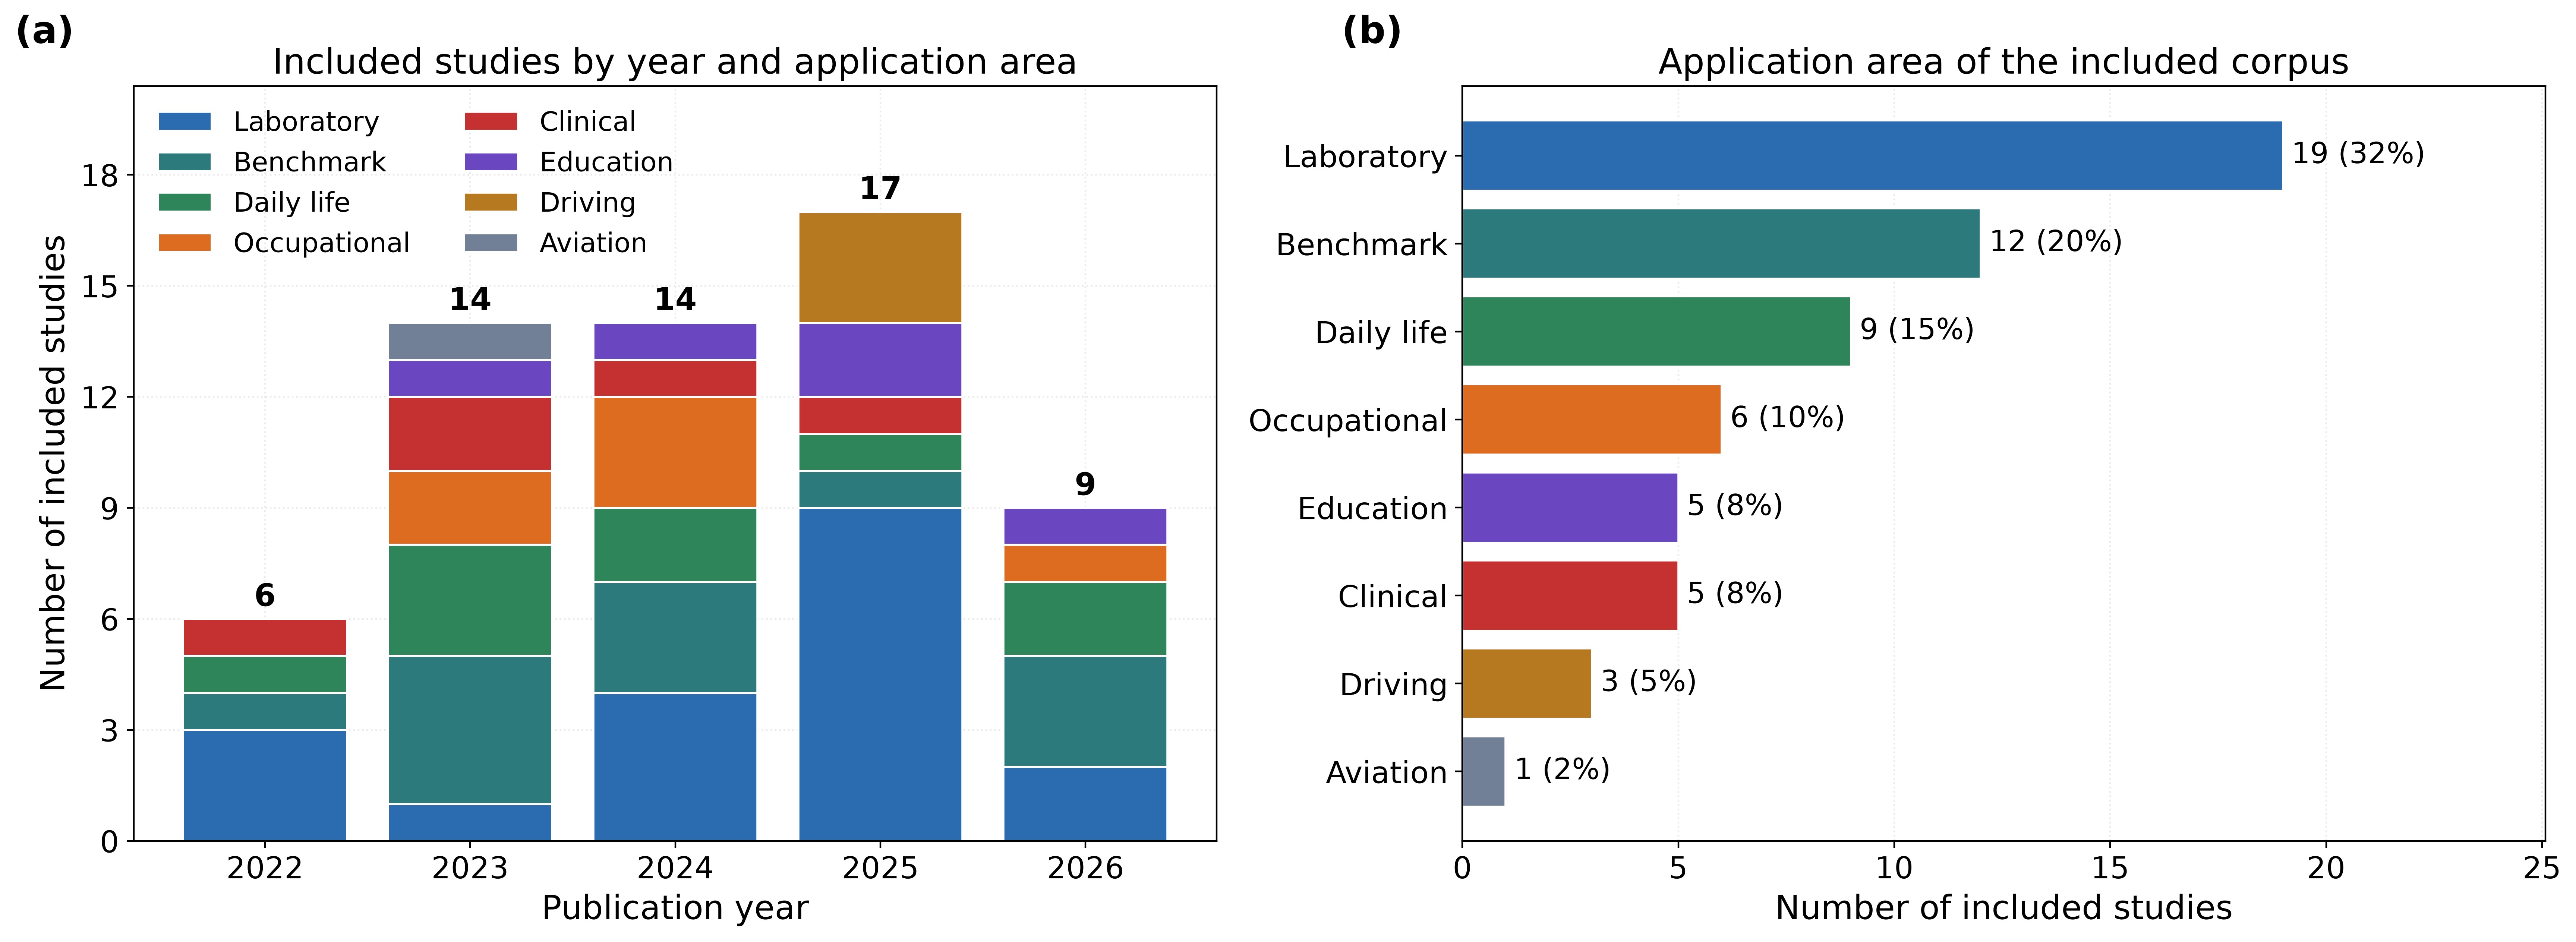
\includegraphics[width=0.99\textwidth]{../figures/fig3_corpus.png}
\caption{Composition of the included corpus. Figure~\ref{fig:corpus}(a) shows the number of
included studies per publication year, with each bar decomposed by application area and the
annual total printed above the bar. Figure~\ref{fig:corpus}(b) shows the total number of
included studies in each application area with the corresponding percentage of the corpus.}
\label{fig:corpus}
\end{figure}

Figure~\ref{fig:screen} summarizes the screening outcome. Figure~\ref{fig:screen}(a) shows the
number of records excluded under each eligibility criterion, and Figure~\ref{fig:screen}(b)
shows the publisher of record for the included studies. Out-of-scope outcomes account for 41
of 56 exclusions (73\%), which quantifies how much of the material customarily cited in this
area does not in fact report a stress or attention outcome.

\begin{figure}[H]
\centering
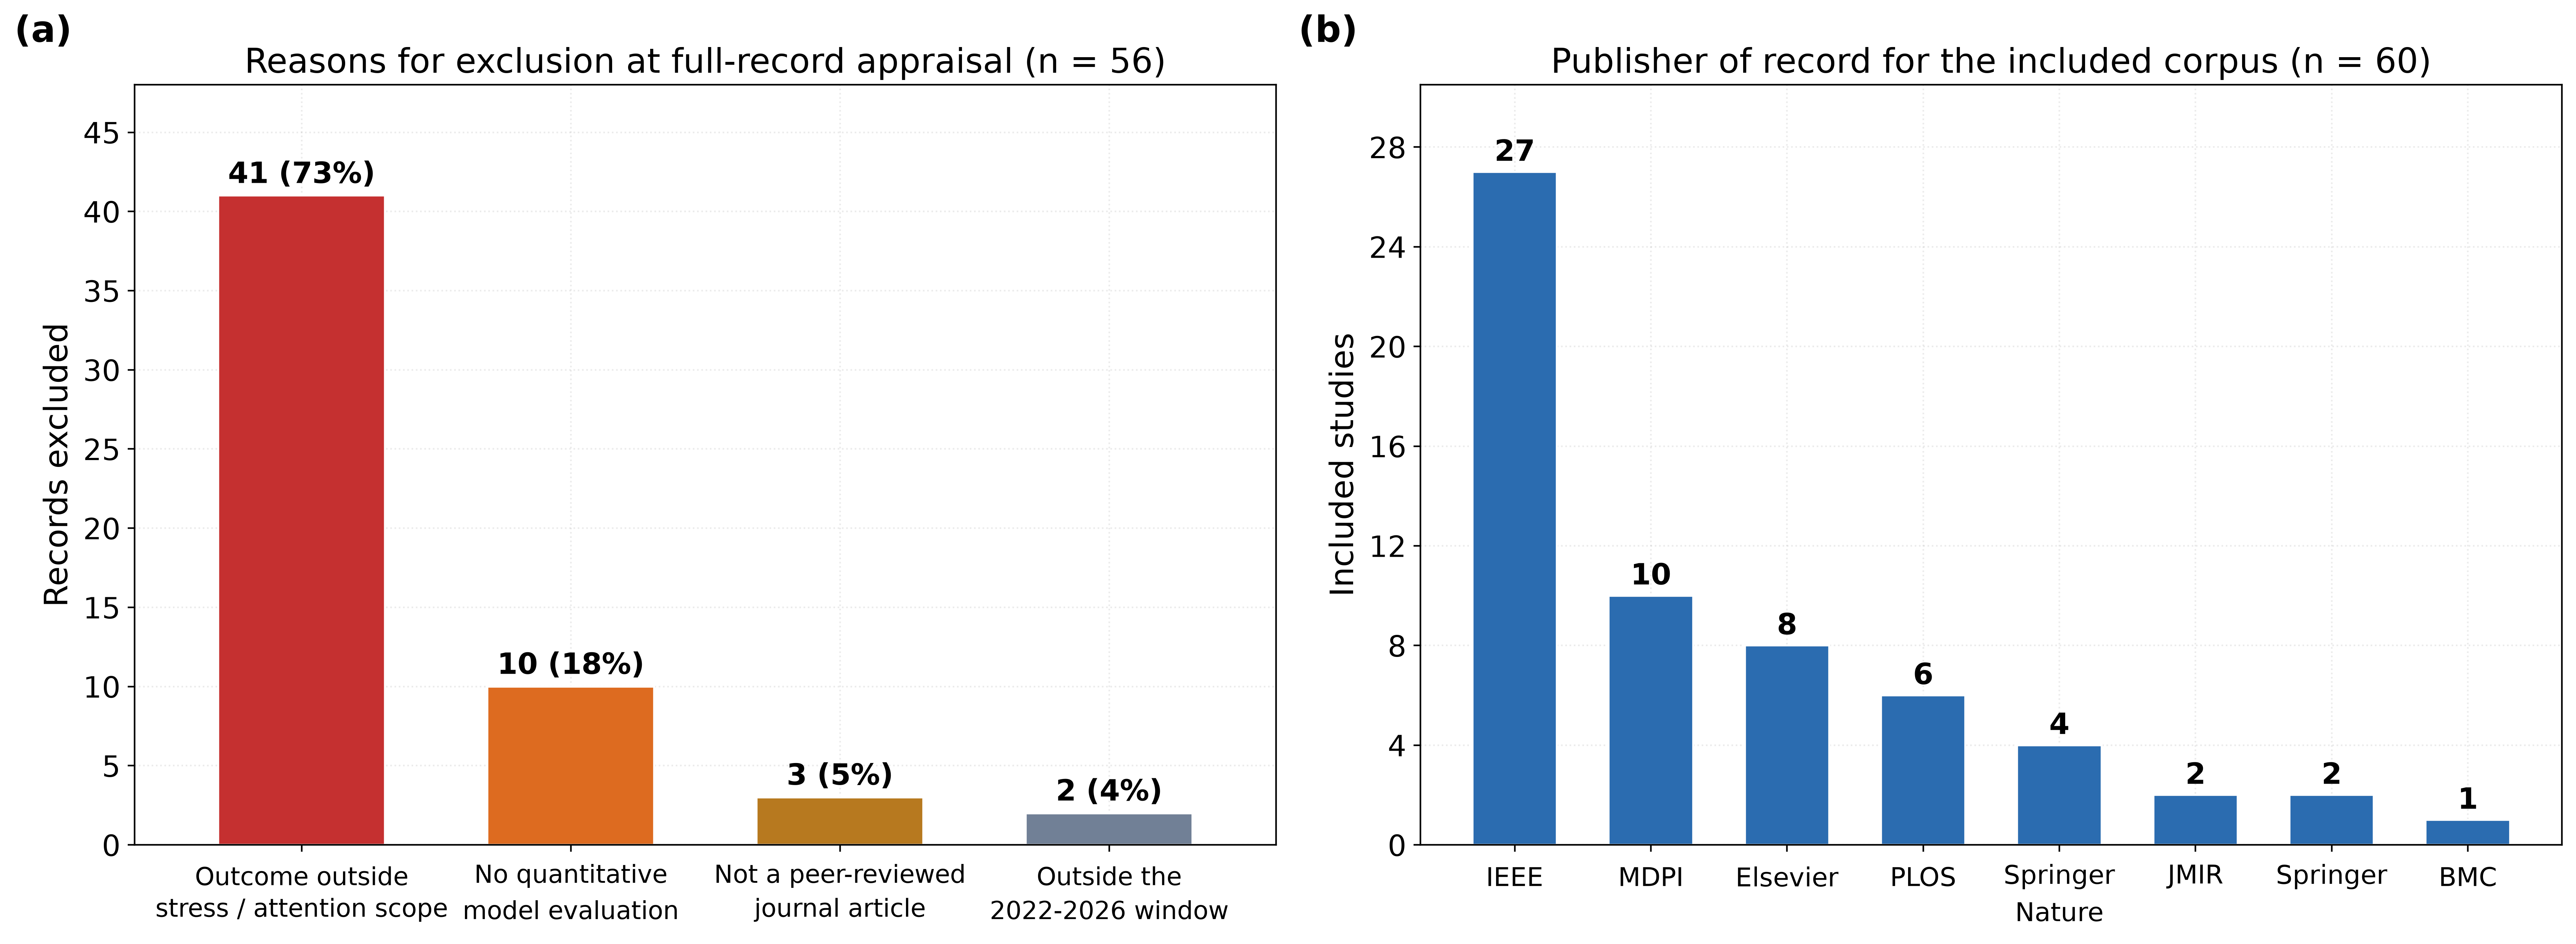
\includegraphics[width=0.99\textwidth]{../figures/fig4_screening.png}
\caption{Screening outcome and corpus provenance. Figure~\ref{fig:screen}(a) shows the number
of records excluded under each eligibility criterion, with the percentage of all exclusions
annotated. Figure~\ref{fig:screen}(b) shows the publisher of record for the 60 included
studies.}
\label{fig:screen}
\end{figure}

\subsection{Reporting Appraisal}
In place of a generic quality checklist, each included study was appraised on whether five
items material to interpreting a reported result could actually be recovered: the headline
performance metric, the size of the evaluation cohort, the validation protocol, whether a
public benchmark was used, and whether any variance or confidence interval accompanied the
point estimate. These items were chosen because each is necessary to decide whether a
reported number transfers. Results are given in Table~\ref{tab:t3} and analyzed in
Section~4.4.

\begin{table}[H]
\centering
\caption{Recovery of reporting items across all 60 included studies. An item is counted as
recovered only where it was explicitly obtained from the openly retrievable record during
verification. Rates therefore bound, from below, how completely this evidence base can be
interpreted by a reader without subscription access.}
\label{tab:t3}
\small
\resizebox{\textwidth}{!}{\begin{tabular}{L{5.4cm} C{2.6cm} C{2.6cm} C{3.1cm}}
\toprule
\textbf{Reporting item} & \textbf{Recovered ($k$)} & \textbf{Not recovered} & \textbf{Recovery rate (\%)} \\
\midrule
Headline metric & 28 & 32 & 46.7 \\
Evaluation cohort size & 18 & 42 & 30.0 \\
Validation protocol & 8 & 52 & 13.3 \\
Public benchmark used & 14 & 46 & 23.3 \\
Variance or CI reported & 3 & 57 & 5.0 \\
\bottomrule
\end{tabular}}
\end{table}

\subsection{Synthesis Strategy}
Two estimands are defined. The \textbf{fusion gain} is the difference, within one study,
between the best single-modality result and the multimodal result obtained on the same
cohort, with the same pipeline and under the same validation protocol. The
\textbf{evaluation-induced gap} is the difference, within one study, between the most
favorable and the most realistic evaluation condition reported for the same model, where
the varied factor is personalization, deployment setting, dataset or task granularity.

Restricting both estimands to within-study contrasts removes the between-study confounds of
cohort, stressor, labeling and preprocessing, at the cost of a small number of eligible
contrasts. Given that $k$, effect sizes are summarized by the median and full range rather
than by a pooled random-effects estimate, and no significance testing is performed; the
comparison of interest is the relative magnitude of two medians, not a hypothesis test.
Accuracy and AUROC differences are both expressed in percentage points (pp) and are reported
separately by metric in the tables so that no cross-metric arithmetic is implied.
